\section{Vistas del prototipo}	
\begin{itemize}
	\item {Vista nueva búsqueda tópico}: Esta vista presenta una barra de búsqueda para ingresar las palabras claves del tópico, la fecha inicial del tópico y un select box para la ubicación del suceso. 
	\begin{figure}[H]
		\centering
		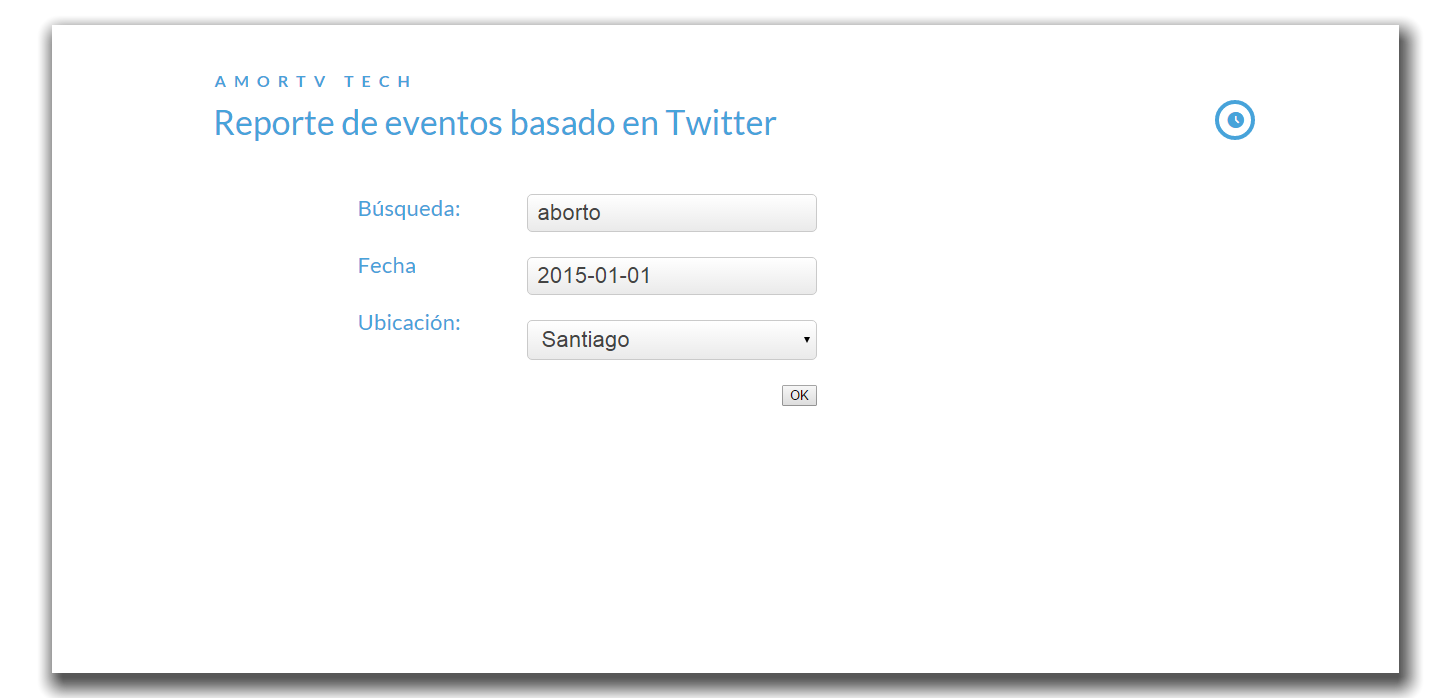
\includegraphics[width=0.9\textwidth]{imgs/vistas_newsearch.PNG}
		\caption{Vista nueva búsqueda tópico}
		\label{fig:vista_newsearch}
	\end{figure}
	
	\item {Vista resultados tweets para nuevo tópico}: Esta vista incluye la cantidad de tweets relacionados al tópico que contabilizó el algoritmo.
	\begin{figure}[H]
		\centering
		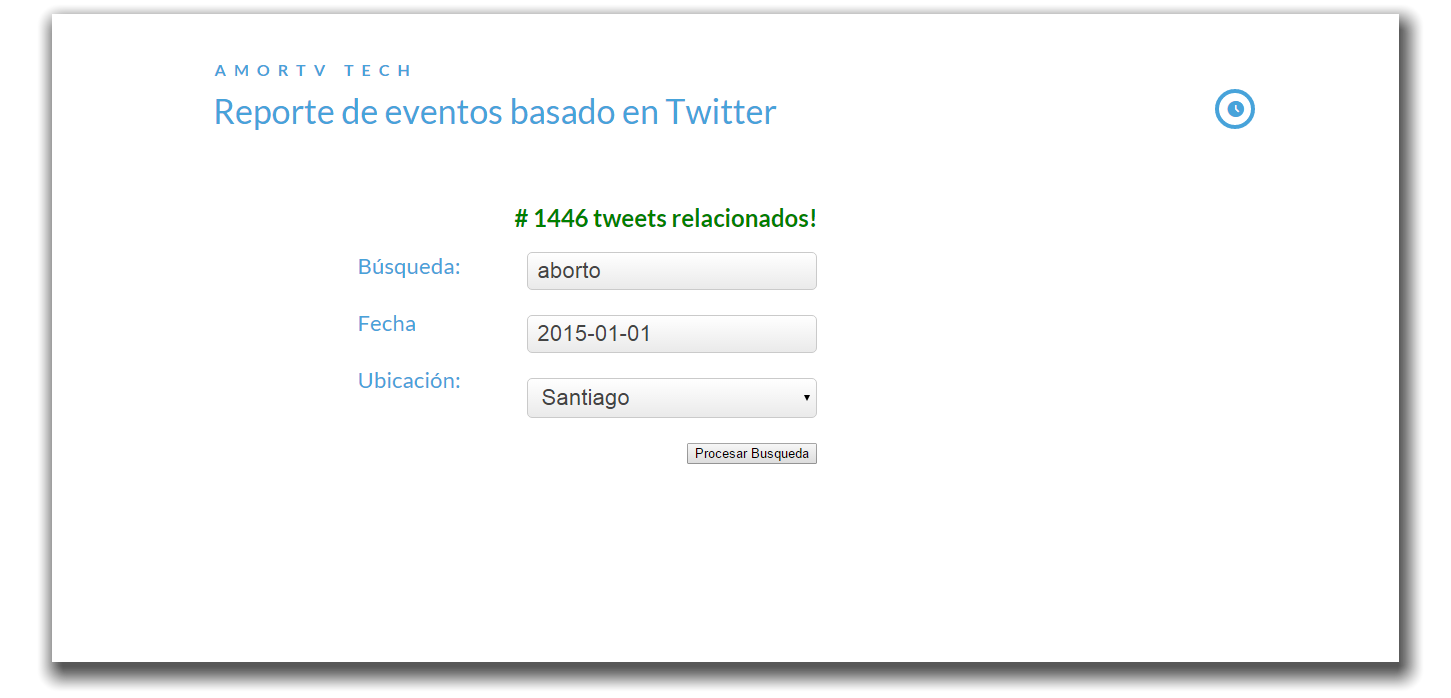
\includegraphics[width=0.9\textwidth]{imgs/vistas_newsearch_results.PNG}
		\caption{Vista resultados tweets para nuevo tópico}
		\label{fig:vista_newsearch_resultados}
	\end{figure}
	\newpage
		\item {Vista tópicos}: Esta vista presenta la lista de los tópicos que han sido buscados previamente, en cada tópico se indica distintas características del tópico: cantidad de tweets, fecha de inicio y ubicación.
		\begin{figure}[H]
			\centering
			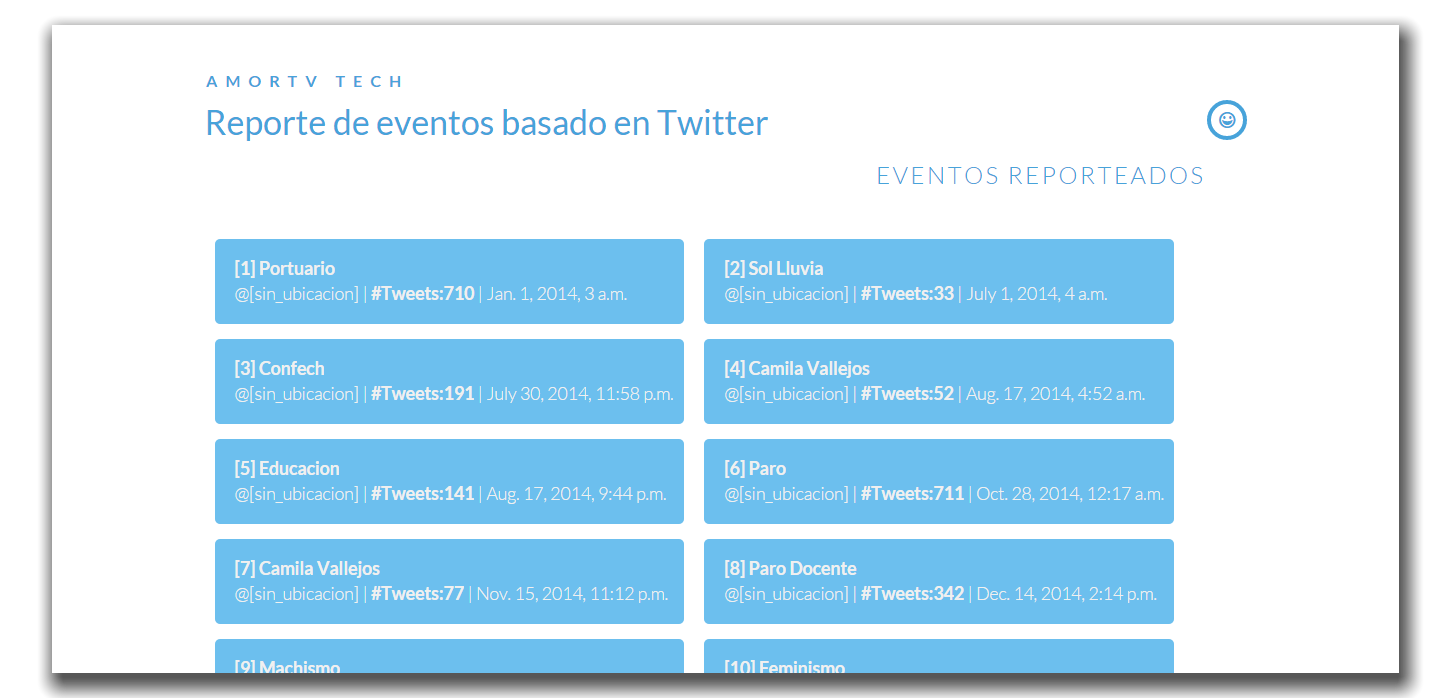
\includegraphics[width=0.9\textwidth]{imgs/vistas_topicos.PNG}
			\caption{Vista de tópicos}
			\label{fig:vista_topicos}
		\end{figure}
	
	\item {Vista orden geográfica}: Esta vista presenta un listado de los tweets relacionados en orden geográfico, en la parte superior de la lista están los tweets emitidos en la ubicación del tópico mientras que en la parte inferior de la lista están los tweets emitidos en la comuna más distante físicamente de la ubicación del tópico.
	\begin{figure}[H]
		\centering
		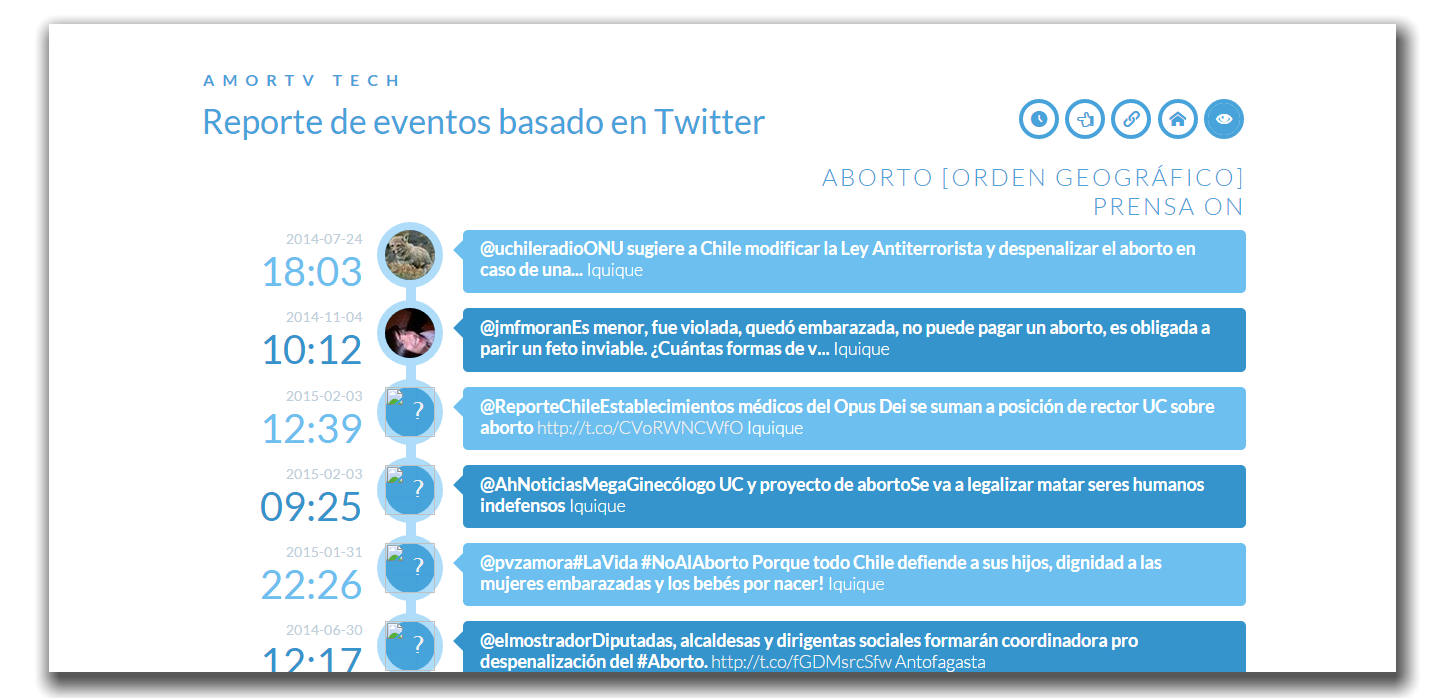
\includegraphics[width=0.9\textwidth]{imgs/vistas_geo.PNG}
		\caption{Vista de orden geográfico}
		\label{fig:vista_geo}
	\end{figure}
	
	\item {Vista orden por relevancia}: Esta vista presenta un listado de los tweets relacionados en orden descendiente por relevancia.
	\begin{figure}[H]
		\centering
		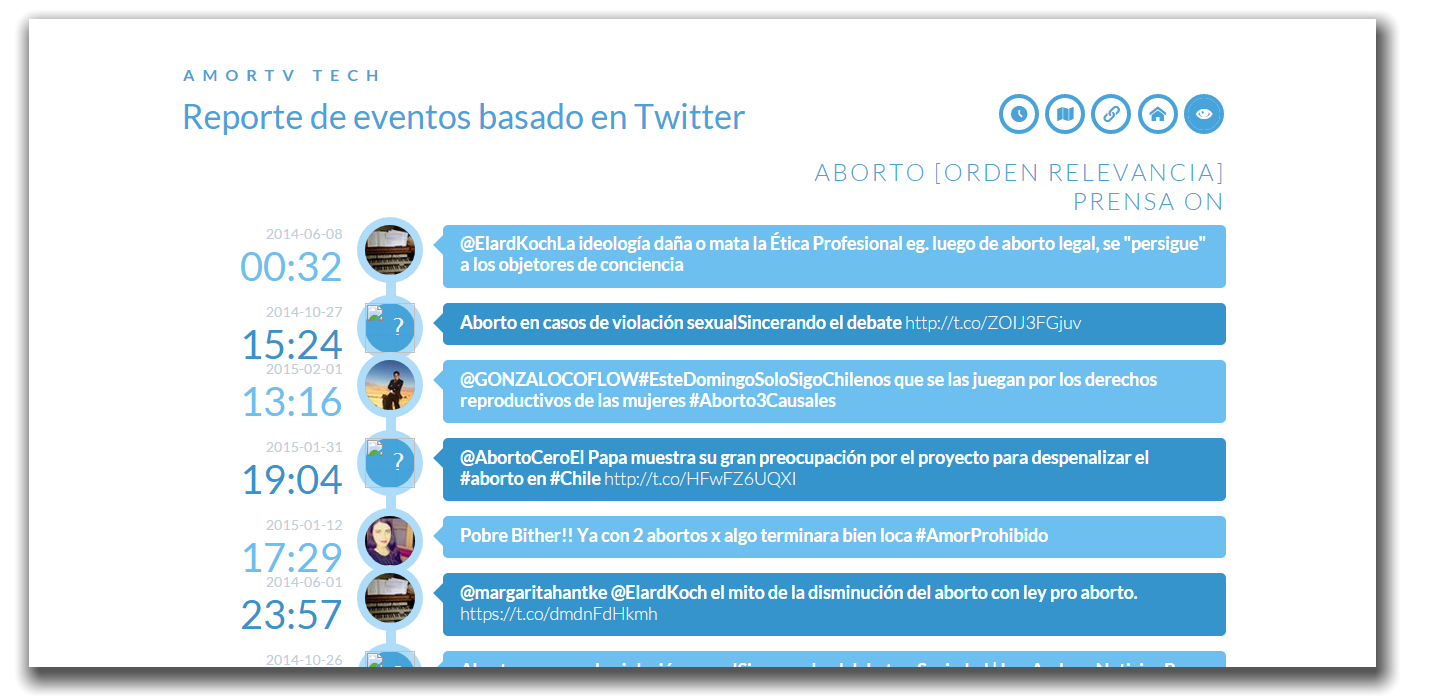
\includegraphics[width=0.9\textwidth]{imgs/vistas_rel.PNG}
		\caption{Vista de orden por relevancia}
		\label{fig:vista_rel}
	\end{figure}
		
	\item {Vista orden temporal}: Esta vista presenta un listado de los tweets relacionados en orden descendiente de fecha de emisión.
	\begin{figure}[H]
		\centering
		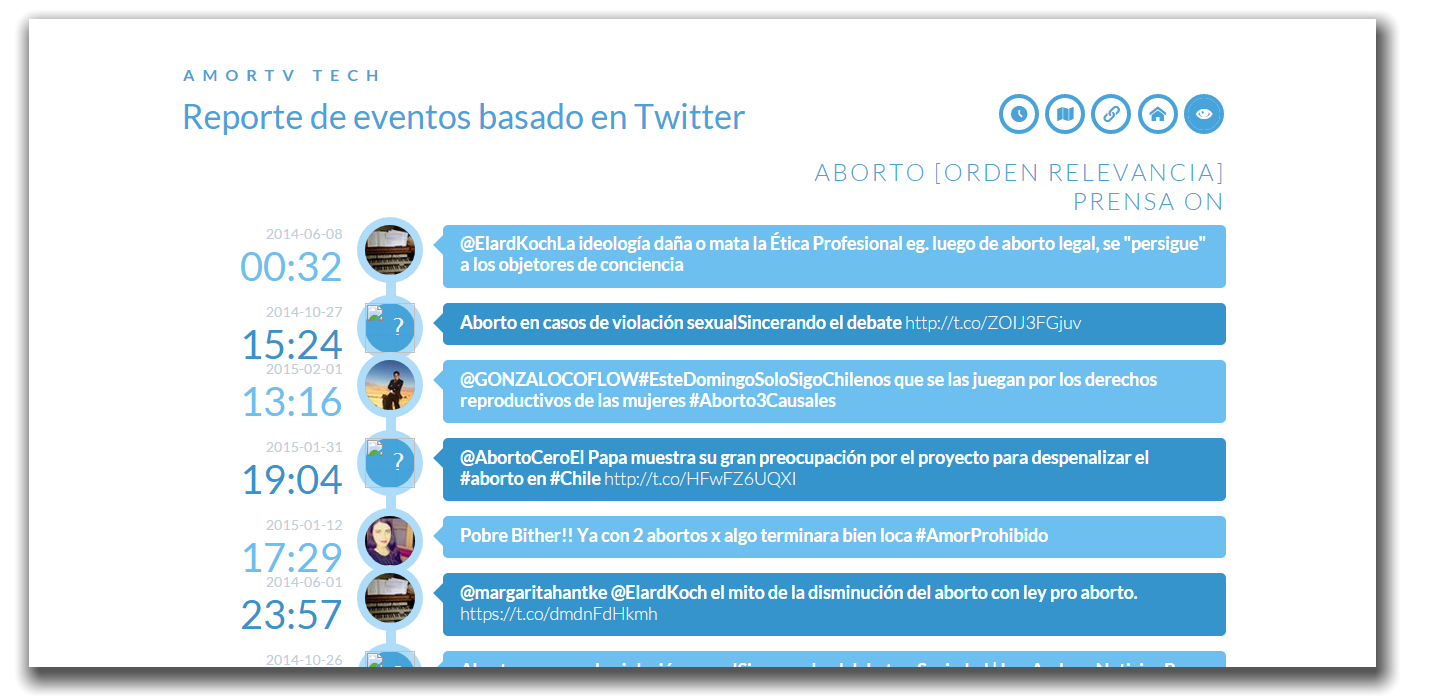
\includegraphics[width=0.9\textwidth]{imgs/vistas_rel.PNG}
		\caption{Vista de orden temporal}
		\label{fig:vista_temp}
	\end{figure}
	
	\item {Vista links}: Esta vista presenta un listado de los enlaces externos contenidos en los distintos tweets relacionados con el tópico, cada una de las casillas presenta una imagen previa del contenido y el titulo del contenido del enlace. Las casillas blancas mostradas en la imagen corresponden a que la imagen previa no pudo ser obtenida.
	\begin{figure}[H]
		\centering
		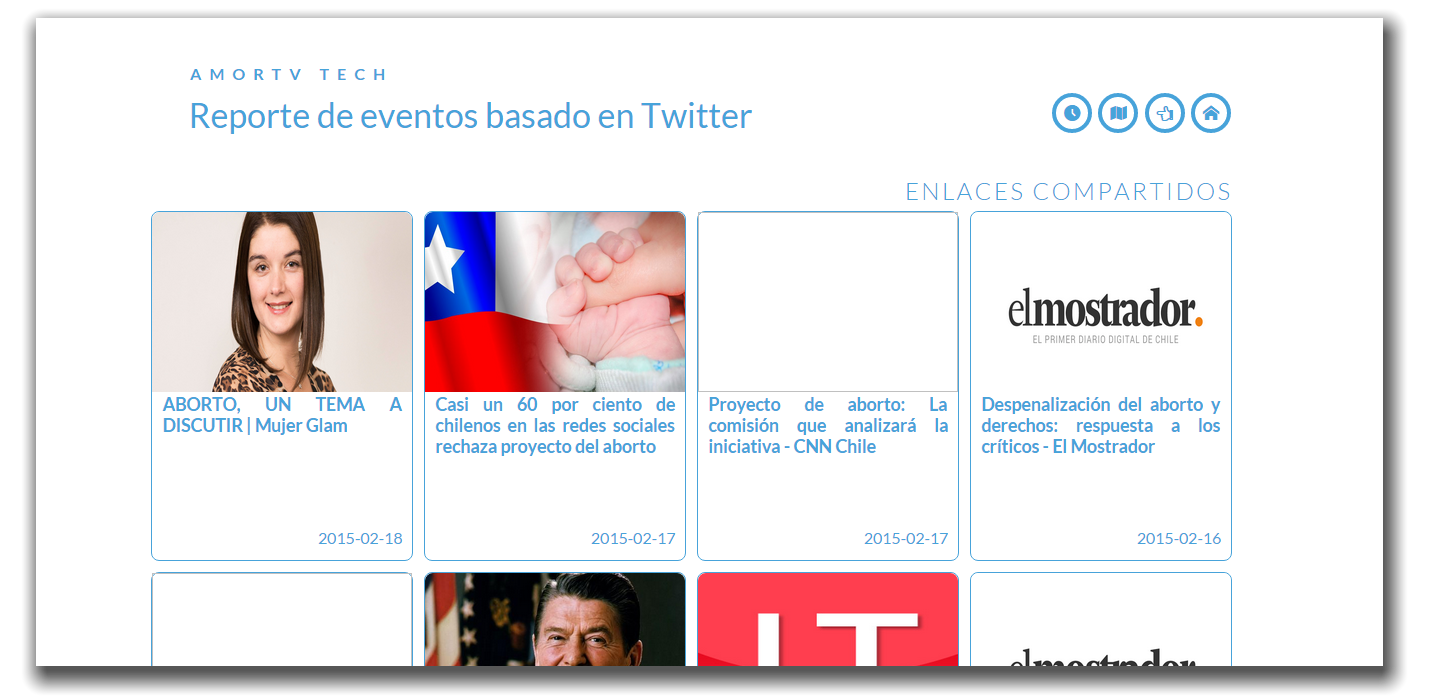
\includegraphics[width=0.9\textwidth]{imgs/vistas_links.PNG}
		\caption{Vista de links}
		\label{fig:vista_links}
	\end{figure}
		
	\item {Botón ON/OFF Prensa}: Este botón oculta o muestra los tweets emitidos por las cuentas identificadas como medio de prensa.
	\begin{figure}[H]
		\centering
		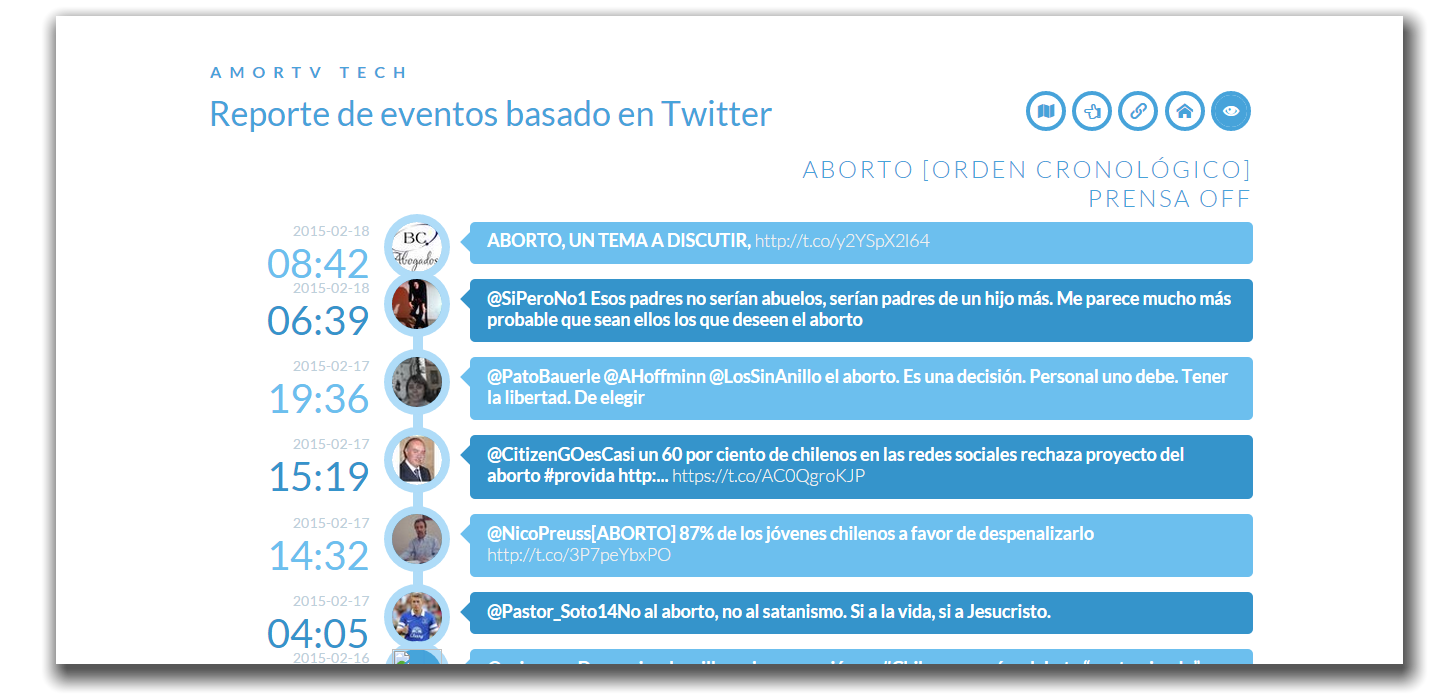
\includegraphics[width=0.9\textwidth]{imgs/vistas_prensa_off.PNG}
		\caption{Vista de tópicos}
		\label{fig:vista_btnprensa_off}
	\end{figure}
	

	
\end{itemize}